\section{レポート課題4}
\subsection{課題1}
\subsubsection{問題}
$10 \times 10$ 分割したマス目内にアトラクタの点が入っているかどうか調べる。点が入っているマス目の数を数えよ。
\subsubsection{解答と考察}
実際にレポート課題4の下にある参考ソースコードを埋め実行してみた。すると[10 34]が出力結果として出てきた。そのためマス目の数は34個である。ソースコードは$N = 1, 2, ..., 500$ までの結果を一括で表示したため最後に掲載する。

\subsection{課題2}
\subsubsection{問題}
$50 \times 50, 100 \times 100, 500 \times 500$ 分割したとき、同様の手順でアトラクタの点が入っているマス目を(プログラムを用いて)数えよ。
\subsubsection{解答と考察}
同様に $N = 50, 100, 500$ で実行した。その結果[50 254], [100 604], [500 4290]がそれぞれ出力された。よってマス目の数は、
\begin{itemize}
  \item $N = 50$ のとき254個
  \item $N = 100$ のとき604個
  \item $N = 500$ のとき4290個
\end{itemize}
となった。また、ソースコードは$N = 1, 2, ..., 500$ までの結果を一括で表示したため最後に掲載する。

\newpage
\subsection{課題3}
\subsubsection{問題}
$N \times N$ 分割したとき上で得た結果が $m \left( N \right)$ だったとする。横軸 $N$ 、縦軸 $m \left( N \right)$ として両対数グラフを描け。何がわかるか。
\subsubsection{画像}
\begin{figure}[htbp]
  \centering
  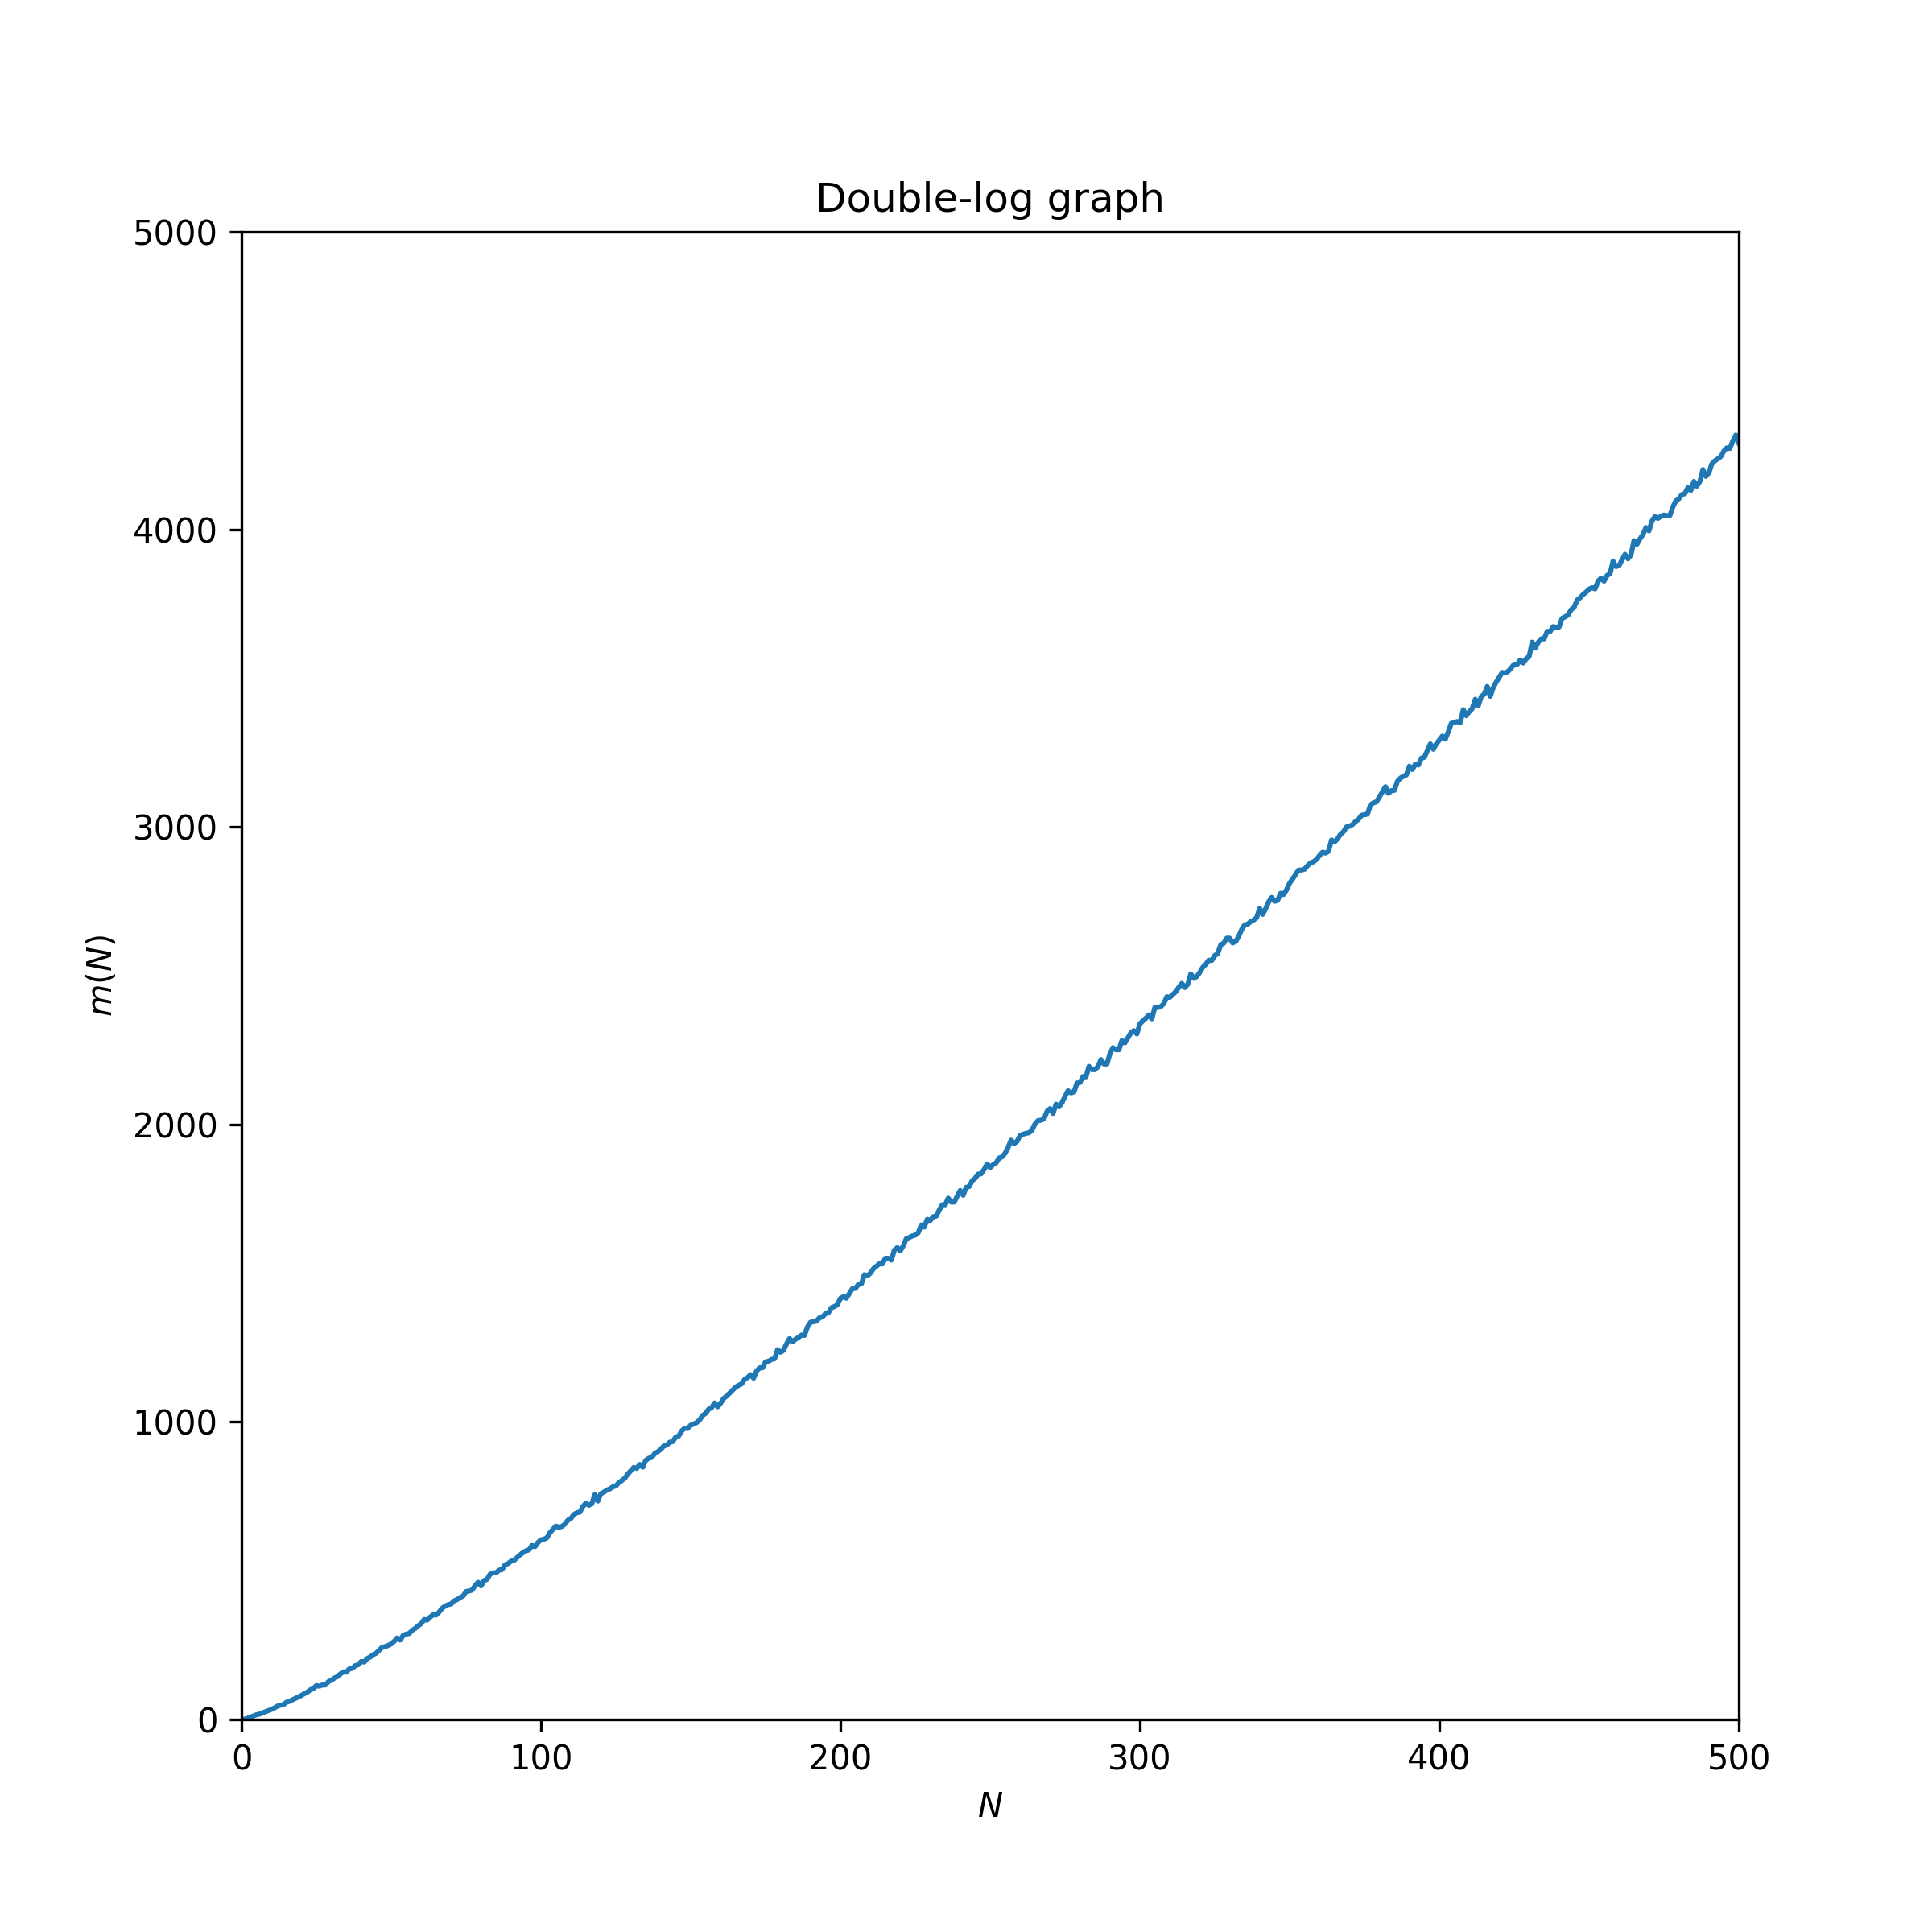
\includegraphics[keepaspectratio, scale=0.5]{images/Problem9/task9.png}
\end{figure}

\subsubsection{考察}
Pythonでは、それぞれの個数を計算するときの計算量に問題があったため、今回は個数計算をC言語グラフの描画をPythonで行った。考察としては、最初のみ直線とは違うような増加の仕方をするが、$N = 50$ あたり以降からは直線的な増加をしていることが挙げられる。


\subsubsection{ソースコード}
\begin{lstlisting}[caption=ctest9.c]
  #include <stdio.h>
  #define N 1000000
  #define nSizeMax 1000

  #define xmin -1.5
  #define xmax 1.5
  #define ymin -0.5
  #define ymax 0.5

  int hist[nSizeMax][nSizeMax];

  void next(double* x, double* y, double a, double b) {
      double xx = (*y) + 1 - a * (*x) * (*x);
      double yy = b * (*x);
      *x = xx;
      *y = yy;
  }

  // initialization
  void init(int nS) {
      int i, j;
      for ( i = 0; i < nS; i++ ) {
          for ( j = 0; j < nS; j++ ) {
              hist[i][j] = 0;
          }
      }
  }

  // print out
  void print(int nS) {
      int i, j, count = 0;
      for ( i = 0; i < nS; i++ ) {
          for ( j = 0; j < nS; j++ ) {
              if (hist[i][j]) {
                  count++;
              }
          }
      }
      printf("%d %d\n", nS, count);
  }


  int main(){
      double a = 1.4, b = 0.3;
      double x = 0.5, y = 0.5;

      for (int nSize = 0; nSize <= 500; nSize++) {
          init(nSize);
          int px, py;
          for (int n = 0; n <= N; n++) {
              next(&x, &y, a, b);
              if (n > 10000) {
                  px = (int)((x - xmin) / (xmax - xmin) * nSize);
                  py = (int)((y - ymin) / (ymax - ymin) * nSize);
                  hist[px][py] = 1;
              }
          }
          print(nSize);
      }
      return 0;
  }
\end{lstlisting}

\begin{lstlisting}[caption=task9.py]
  from matplotlib import pyplot as plt
  import numpy as np

  filepath = '複雑系科学演習/Week9/ctest9.txt'
  x_array = []
  y_array = []
  with open(filepath, encoding='UTF-8') as f:
      while line := f.readline():
          line = line.rstrip()
          x, y = line.split(' ')
          x_array.append(int(x))
          y_array.append(int(y))

  plt.figure(figsize=(8, 8))
  plt.xlim(0, 500)
  plt.ylim(0, 5000)
  plt.plot(x_array, y_array)
  plt.title('Double-log graph')
  plt.xlabel('$N$')
  plt.ylabel('$m(N)$')
  # plt.show()
  plt.savefig('複雑系科学演習/Week9/images/task9', dpi=300)
\end{lstlisting}